\documentclass{article}
\usepackage[utf8]{inputenc}
\usepackage[icelandic]{babel}
\usepackage[T1]{fontenc}
\usepackage{graphicx}
\usepackage{mathtools}
\usepackage{amsmath}
\usepackage{amssymb}
\usepackage{minted}


\graphicspath{ {./} }
\title{Calendar - Viðmótsforritun}
\author{ttb3@hi.is}
\date{\today}


\begin{document}
\maketitle


\section*{Keyrsla}
\begin{center}
    
\includegraphics[scale=0.3]{imgs/s1.png}\\
    fyrst þegar forritið er keyrt\\
    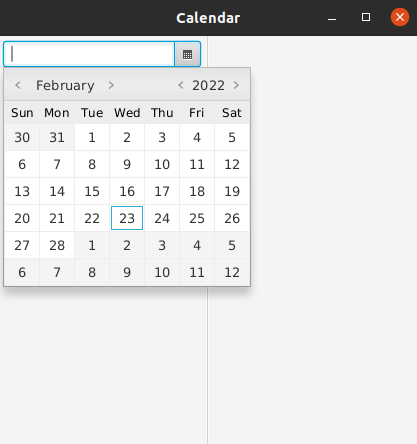
\includegraphics[scale=0.3]{imgs/s2.png}\\
    þegar smellt er á dagatalið, hægt að sjá hvaða dagur er í dag með litla bláa border\\
    
\includegraphics[scale=0.3]{imgs/s3.png}\\
    dagur valinn, dagsetning sést efst\\
    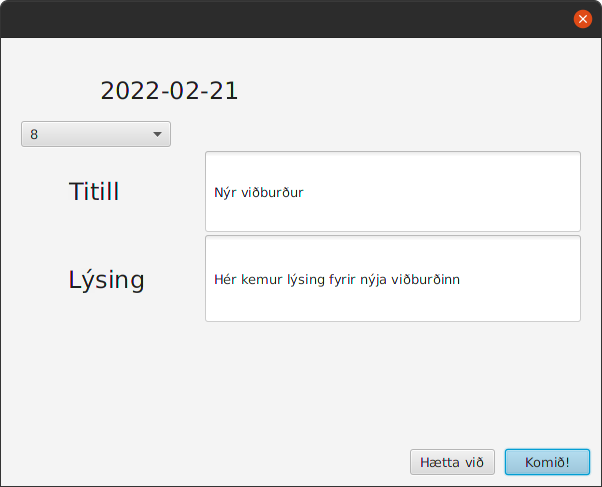
\includegraphics[scale=0.3]{imgs/s4.png}\\
    ef tvísmellt er ehvstaðar á daginn kemur event creatorinn upp\\
    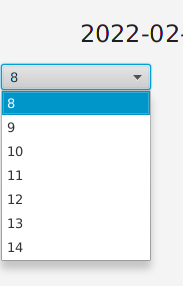
\includegraphics[scale=0.3]{imgs/s5.png}\\
    þar er hægt að breyta titli, lýsingu og velja hvenær viðburður byrjar með dropdown menu\\
    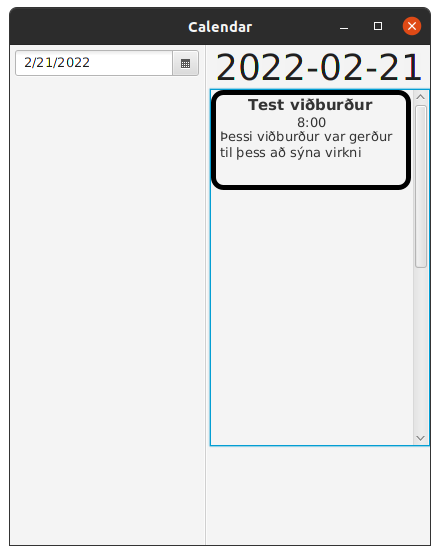
\includegraphics[scale=0.3]{imgs/s6.png}\\
    þarna er viðburðurinn tilbúinn\\
    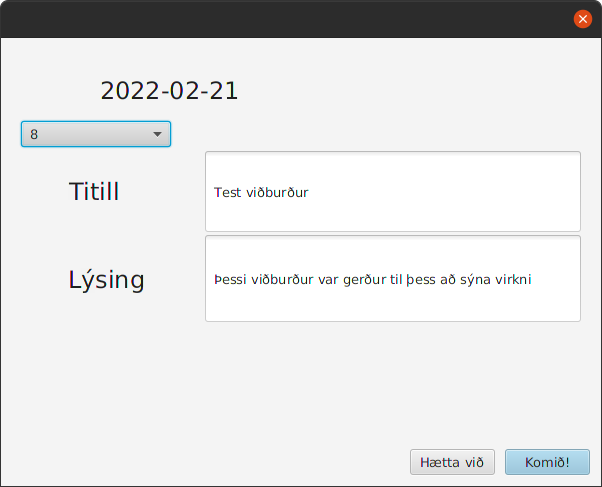
\includegraphics[scale=0.3]{imgs/s8.png}\\
    svo er hægt að tvísmella á viðburðinn sjálfan til að fá upp event editorinn\\
    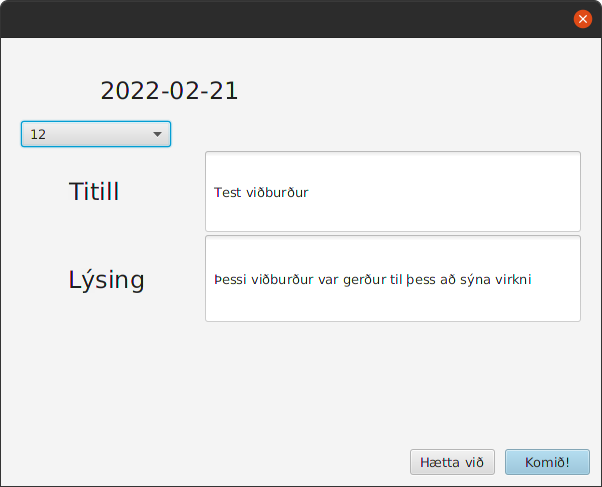
\includegraphics[scale=0.3]{imgs/s9.png}\\
    þarna breytti ég bara hvenær viðburðinn byrjaði\\
    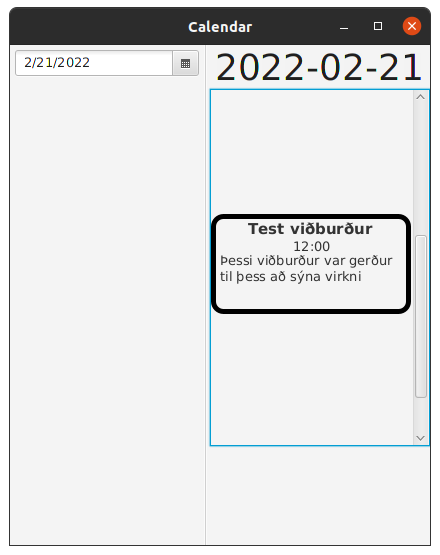
\includegraphics[scale=0.3]{imgs/s11.png}\\
    þá færist viðburðurinn niður miðað við byrjunartíma\\
    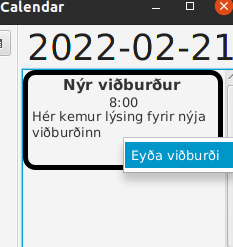
\includegraphics[scale=0.3]{imgs/s12.png}\\
    svo er hægt að hægrismella til að eyða viðburðinum\\
    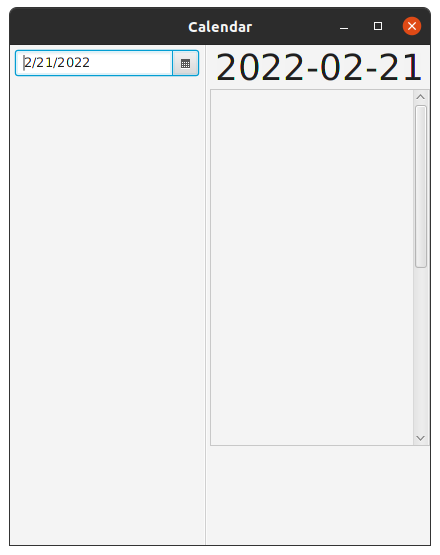
\includegraphics[scale=0.3]{imgs/s13.png}\\
    viðburðurinn farinn :)
\end{center}




\end{document}